\chapter{Related Work} \label{related}
\section{3D Druck und Additive Fertigung von Gebäuden}
\section{Legeroboter}
\subsection{Digital Plan of Brickwork Layout for Robotic Bricklaying Technology}
In diesem Paper stellen Usmanov et al. ein generelles Vorgehen für das Erstellen eines Ziegel-Legeplans für ein als digitales Modell vorliegendes Gebäude vor \cite{Usmanov2021}.
Dieses Vorgehen gliedern sie in sechs Schritte:
\begin{enumerate}
\item Das vorliegende IFC Modell (siehe \ref{basics:ifc}) nach Wandelementen durchsuchen und diese in das sogennante BREP-Format (siehe \ref{basics:brep}) konvertieren.
\item Das Aufteilen des gesamten Modells in Schichten, die der Modulhöhe des verwendeten Ziegelsteinformats entspricht.
\item Verbindungen von getrennt modellierten Wandelementen heraussuchen. Dies ist zum Beispiel an Eckstücken der Fall, da dafür oft zwei einzelne Wandelemente modelliert werden, welche in einem Winkel zueinander stehen und sich berühren. Für die nachfolgenden Schritte sind diese Verbindungen relevante Informationen.
\item  Mit den Informationen der vorhergegangenen Schritte können nun für jede Schicht kritische Bereiche identifiziert werden, an welchen später ein komplexer Legevorgang von Ziegeln von Nöten ist.
\item  Nun werden zunächst die kritischen Bereiche anhand einer vorher definierten Legeanleitung mit teilweise angepassten Ziegelsteinen bestückt und im Anschluss die restlichen Bereiche aller Wände mit dem ausgewählten Standardziegel aufgefüllt. In diesem Schritt werden zusätzlich Fenster- und Türstürze über deren Öffnungen in den Wänden gelegt.
\item Dieser Schritt fasst das Anzeigen als 3D Modell und Konvertieren des Resultats in eine nicht konkreter definierte Listenform zusammen. Das Ergebnis für das von den Autoren ausgewählte Beispielgebäude ist in Abbildung \ref{fig:usmanov} zu sehen.
\end{enumerate}

\begin{figure}[ht]
    \centering
    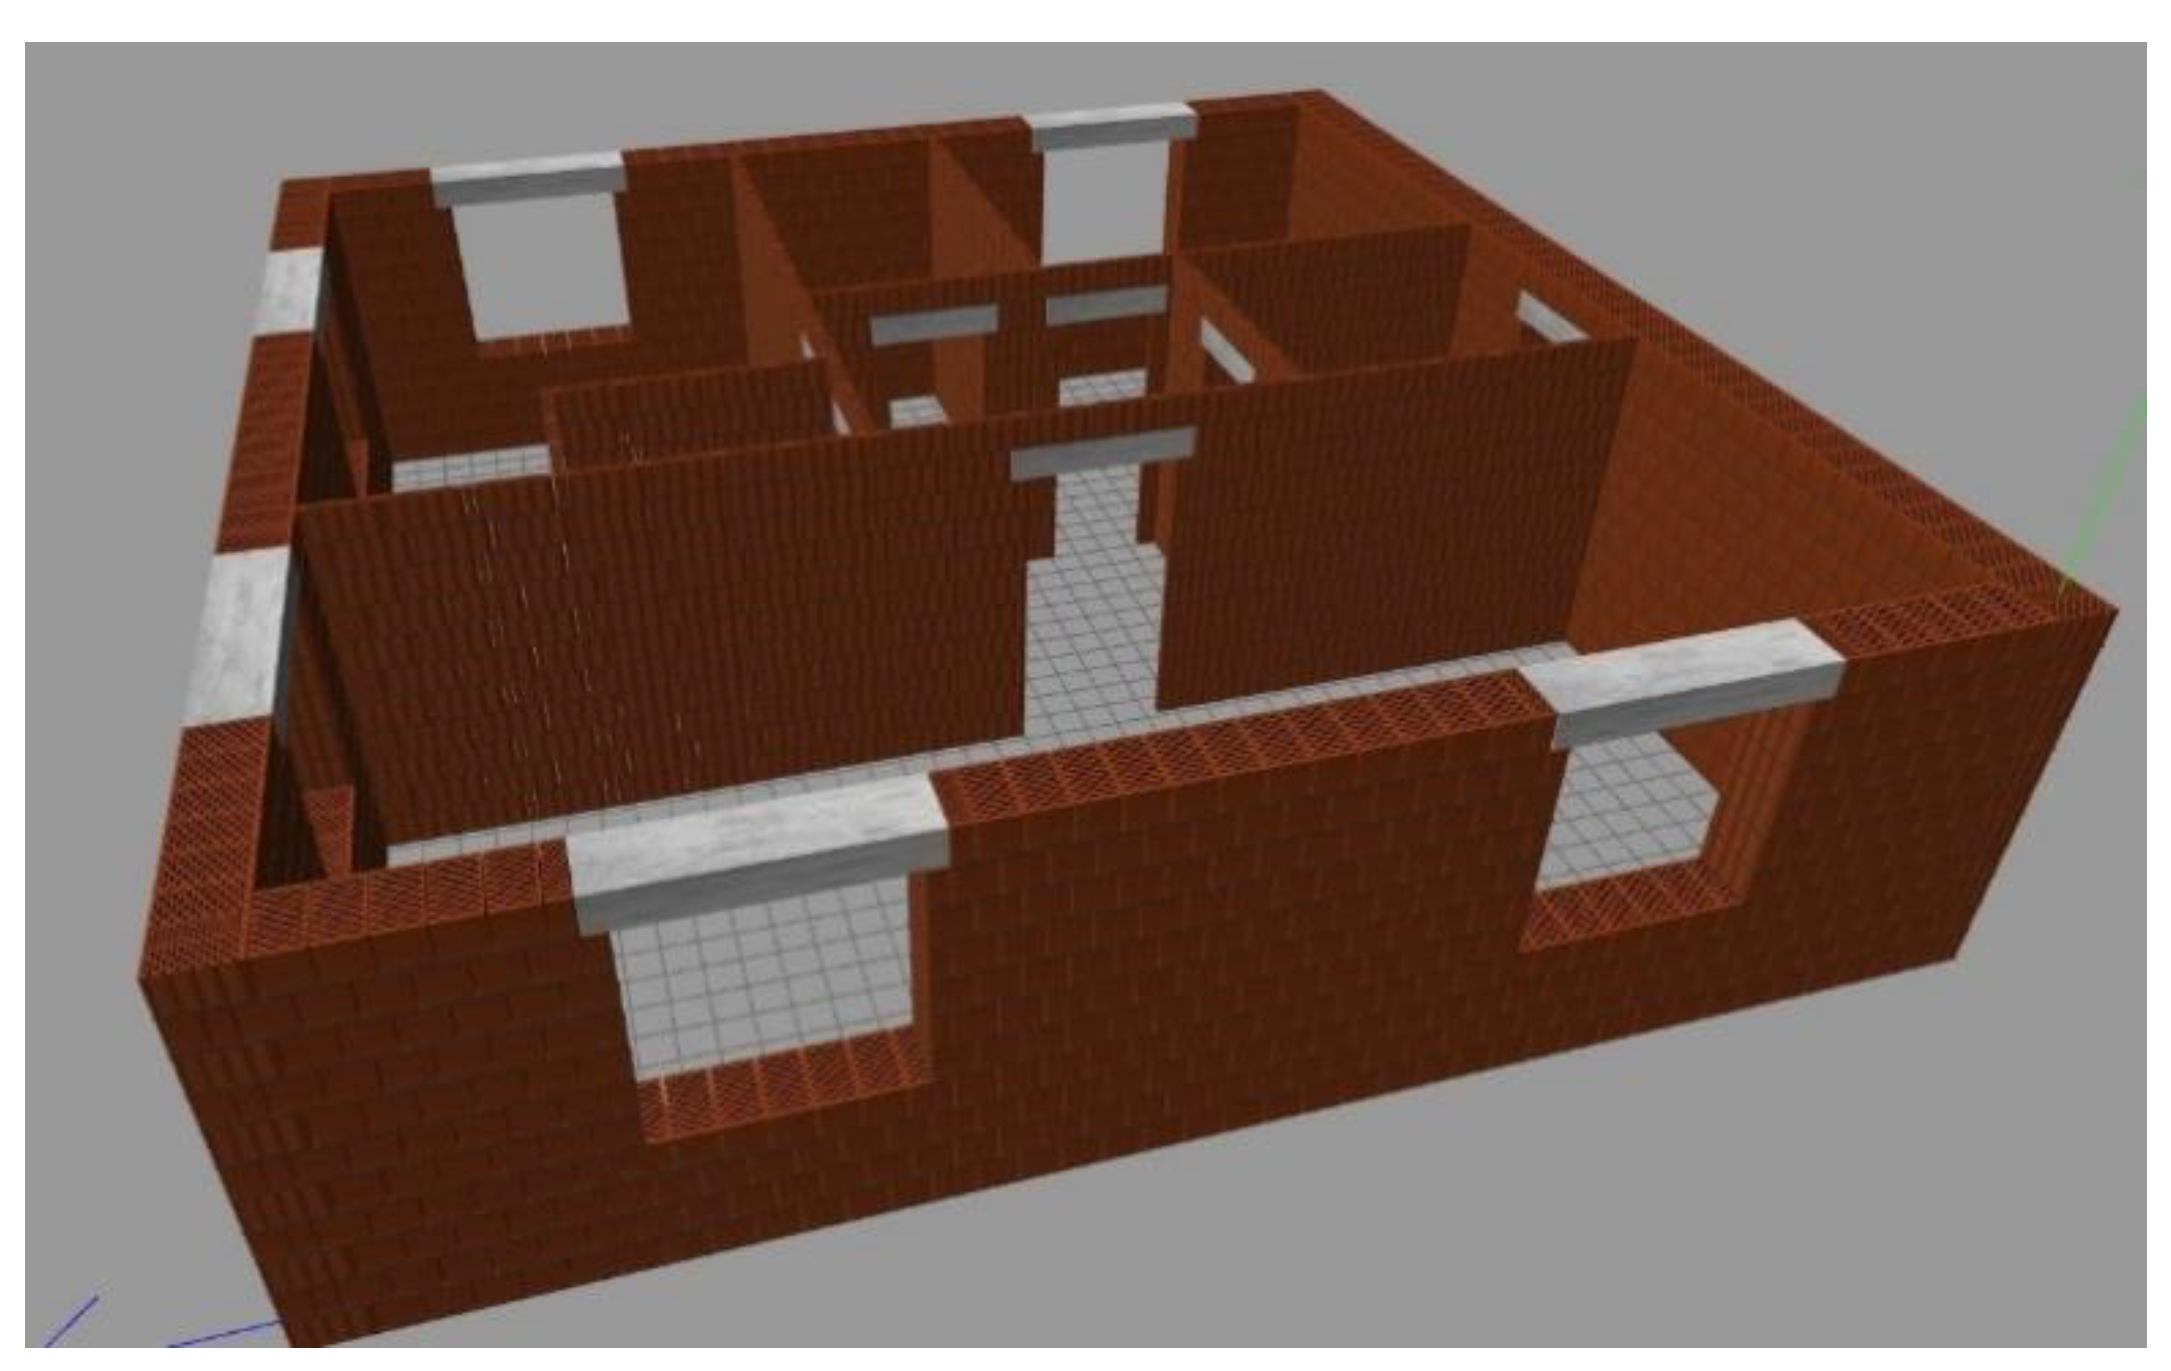
\includegraphics[width=0.6\columnwidth]{fig/sustainability-13-03905-g004.png}
    \caption{Ergebnis des Verfahrens zur Erstellung eines Ziegel-Legeplans nach Usmanov et al. \cite{Usmanov2021}.}
    \label{fig:usmanov}
\end{figure}

Besonders detailliert ist ihr Ansatz für das Finden von besagten kritischen Teilbereichen einer Wand mithilfe einiger mathematischer Gleichungen, die alle Wände zueinander in Beziehung stellen.
Diese Teilbereiche sind Wandecken, T-Kreuzungen (wie etwa der Übergang einer Innenwand an eine Außenwand) und Öffnungen innerhalb einer Wand und sind ebenfalls in Kapitel \ref{scenarios:scenario1:problem} dieser Arbeit als Problemstellung aufgeführt.
Anhand der von ihnen zusammengetragenen Informationen konnten die Autoren erfolgreich die bestmögliche Platzierung von vier Roboterarmen errechnen, die den schnellstmöglichen Bau des Gebäudes ermöglichen.
Dennoch werden zum Schluss noch einige Einschränkungen ihres Verfahrens angesprochen.
Vor allem die Beschränkung auf 90 Grad Ecken und das Gebunden sein an einen einzigen Standardziegel werden als besonders restriktiv wahrgenommen.

Insbesondere die Verwendung von verschiedenen Ziegelformaten und das algorithmische Finden von Lösungen an den kritischen Teilbereichen einer Wand, anstatt diese als Legeplan vorliegen zu haben, sind Ziele dieser Arbeit.
Dennoch sind einige Punkte ihres Vorgehens auch zwangsläufig notwendige Schritte für diese Arbeit und werden in einer ähnlichen Form vorzufinden sein.

\section{Materialien}
\section{Bausteine}
\section{Wall detailing und das (3D) Bin Packing Problem}
\label{basics:wall-detailing}
TODO hinführen über Bin Packing hin zu "spezialfall" Wall detailing mit arbiträren Bausteinen und Eigenschaften (wie versetzen der ziegel)

TODO über bin packing schreiben, erklären paper suchen, lösungsansätze zu np hartem problem 

Xu Chengran et al. haben in ihrem Paper "Optimal brick layout of masonry walls based on intelligent evolutionary algorithm and building information modeling" verschiedene Optimierungsansätze aus dem Bereich des 2D Packaging Problems getestet \cite{Xu2021}.
%TODO was ist das für ein Problem? Zitat aus nem Paper finden!
Konkret wurden drei Algorithmen verwendet: Differential Evolution, Particle Swarm Optimization und Neighbourhood Field Optimization.
%TODO ergebnisse vergleichen und eines davon hervorheben, welches ich evtl selbst einbau
Außerdem wird ein drei-phasiges Vorgehen vorgeschlagen: Data collection, Brick layout und Data Output.
%TODO das vmtl einfach auch so aufziehen. Mauern aus modell extrahieren mit geometrischen infos, optimieren und iwie rausballern
Dieses Vorgehen eignet sich auch für das Finden von Bausteinkonfigurationen in dieser Arbeit, da zuerst alle relevanten geometrischen Daten (in diesem Fall Wände, Fenster, Türen usw.) aus dem 3D Modell gesammelt werden müssen, bevor das Detailing stattfinden kann.
Nach dem Optimieren der Bausteinkonfiguration muss das Ergebnis ebenfalls in ein Format gebracht werden, das für die folgenden Schritte verwendet und eventuell auch dem Nutzer angezeigt werden kann.


Soft items: https://arxiv.org/abs/2206.15116

Irregular Shaped items: https://link.springer.com/content/pdf/10.1631/FITEE.1400421.pdf

"Parametric Blockwall-Assembly Algorithms for the Automated Generation of Virtual Wall Mockups Using BIM"
\section{Ludwigs Dissertation}
\label{related:ludwigs dis}


%https://www.mdpi.com/2227-7390/7/12/1232
%https://www.mdpi.com/2071-1050/13/7/3905
%https://www.itcon.org/papers/2014_13.content.080704.pdf
%https://books.google.de/books?hl=de&lr=&id=9-HxCwAAQBAJ&oi=fnd&pg=PA257&dq=Autonomous+robotic+building+system&ots=090tO8dB6l&sig=MiaKFiU5uqRUFeEH5rBg08wfvL8#v=onepage&q=Autonomous%20robotic%20building%20system&f=false